\documentclass[tikz,border=3mm]{standalone}
\usepackage[siunitx]{circuitikz}
\usetikzlibrary{calc,positioning,arrows.meta}

\begin{document}

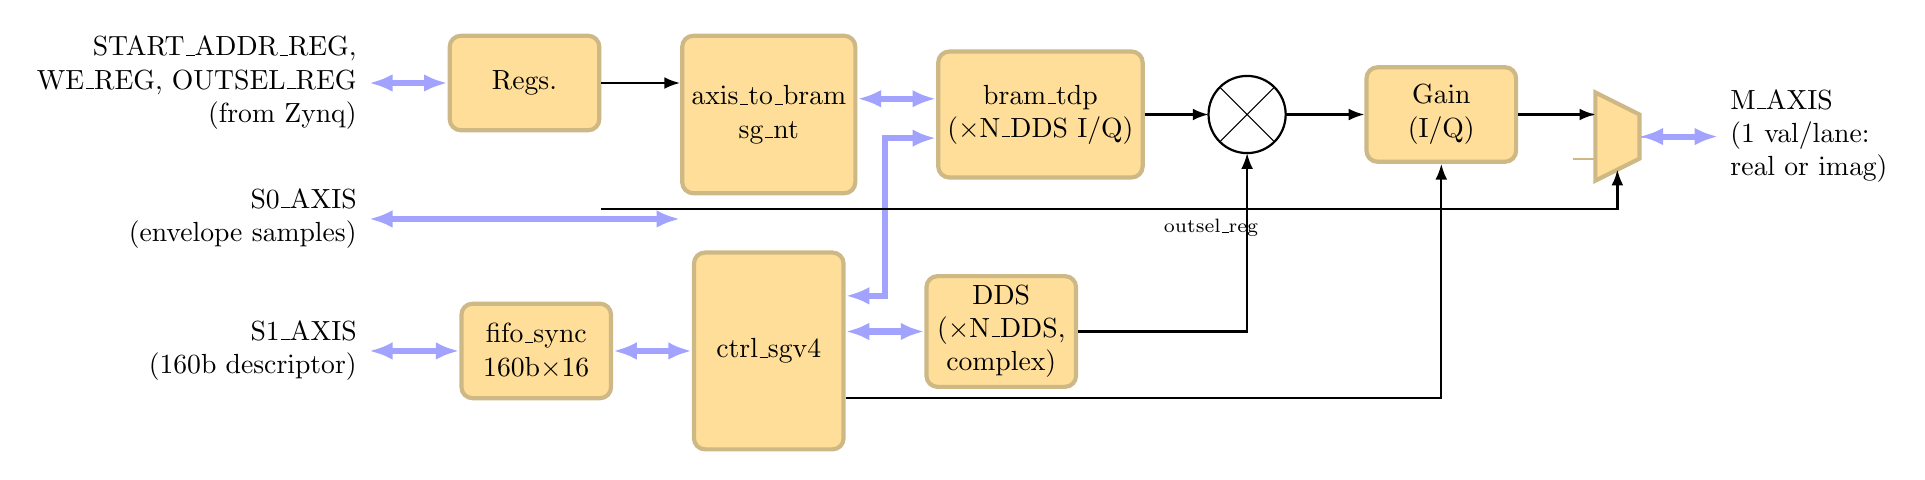
\begin{tikzpicture}
[box/.style={align=center, draw,rounded corners,minimum width=1.9cm,minimum height=1.2cm,draw={rgb,255:red,205; green,184; blue,134},fill={rgb,255:red,254; green,222; blue,152},line width=1.5pt},
arrow/.style={line width=2.2pt,draw={rgb,255:red,162; green,163; blue,255},{Latex[length=3mm]}-{Latex[length=3mm]}},
single arrow/.style={line width=0.8pt,-{Latex[length=2mm]}},
outmux/.style={muxdemux, muxdemux def={Lh=2,NL=2,Rh=1,NR=1,NB=1,w=1},draw={rgb,255:red,205; green,184; blue,134},fill={rgb,255:red,254; green,222; blue,152},line width=0.75pt},
node distance=0.4cm]

% Data writer.
\node[box,minimum height=2cm] (data writer) {axis\_to\_bram\\ sg\_nt};

% Control.
\node[box,below=0.7cm of data writer,minimum height=2.5cm] (ctrl) {ctrl\_sgv4};

% Memory.
\node[box,right=1cm of data writer,minimum height=1.6cm] (mem) {bram\_tdp\\ ($\times$N\_DDS I/Q)};

% DDS (complex).
\coordinate (temp) at ($(ctrl.north east)+(1,-0.3)$);
\node[box,anchor=north west] (dds) at (temp) {DDS\\($\times$N\_DDS,\\ complex)};

% Regs.
\coordinate (temp) at ($(data writer.north west)+(-1,0)$);
\node[box,anchor=north east] (axi regs) at (temp) {Regs.};

% Fifo.
\node[box,left=1cm of ctrl] (fifo) {fifo\_sync\\160b$\times$16};

% Mixer (complex product).
\coordinate (temp) at ($(mem.east)+(1.3,0)$);
\node[mixer] (mixer) at (temp) {};

% Gain (complex, applied before the static select).
\node[box,right=1cm of mixer] (gain) {Gain\\(I/Q)};

% Static real/imag output select.
\coordinate (temp) at ($(gain.east)+(0.7,0)$);
\node[outmux,anchor=lpin 1] (out mux) at (temp) {};

% s_axi (registers).
\draw[arrow] ($(axi regs.west)+(-1,0)$) coordinate (s axi in) node[anchor=east,align=right] {START\_ADDR\_REG,\\WE\_REG, OUTSEL\_REG\\(from Zynq)} -- (axi regs.west);

% s0_axis.
\draw[arrow] ($(s axi in |- axi regs.south)+(0,-1.1)$) coordinate (temp) node[anchor=east,align=right] {S0\_AXIS\\(envelope samples)} -- (temp -| data writer.west);

% s1_axis.
\draw[arrow] (s axi in |- fifo.west) coordinate (temp) node[anchor=east,align=right] {S1\_AXIS\\(160b descriptor)} -- (temp -| fifo.west);

% Regs -> data writer.
\draw[single arrow] (axi regs) -- (axi regs -| data writer.west);

% Data writer -> memory.
\draw[arrow] ($(data writer.east)+(0,0.2)$) coordinate (temp) -- (temp -| mem.west);

% Control -> dds.
\draw[arrow] (dds.west) -- (dds.west -| ctrl.east);

% Control -> memory (mem_addrb).
\draw[arrow] ($(ctrl.east)+(0,0.7)$) -- ++(0.5,0) |- ($(mem.west)+(0,-0.3)$);

% Control -> Fifo (fifo_rd_en).
\draw[arrow] (ctrl) -- (fifo);

% memory -> mixer (envelope, I/Q).
\draw[single arrow] (mem.east) -- (mixer.west);

% dds -> mixer.
\draw[single arrow] (dds.east) -| (mixer.south);

% mixer -> gain.
\draw[single arrow] (mixer.east) -- (gain.west);

% Control -> gain.
\draw[single arrow] ($(ctrl.east)+(0,-0.6)$) -| (gain.south);

% gain -> mux.
\draw[single arrow] (gain.east) -- (out mux.blpin 1);

% Regs -> mux selection (static outsel_reg, not per-descriptor).
\draw[single arrow] ($(axi regs.east)+(0,-1.6)$) -| (out mux.bbpin 1) node[pos=0.3,below,font=\scriptsize] {outsel\_reg};

% m_axis.
\draw[arrow] (out mux.brpin 1) -- ++(1,0) node[anchor=west,align=left] {M\_AXIS\\(1 val/lane:\\ real or imag)};

\end{tikzpicture}

\end{document}
